\scanpage{64}
\mspage{7}
théorie de la représentation conforme, ce disque holomorphe doit être isomorphe au disque \unsure{standart} $\mathbb D$, via un isomorphisme unique
\[
g:\mathbb D\xrightarrow{\sim}f\qquad
\begin{aligned}
0&\longmapsto\infty\quad\text{(centre de $f$)}\\
1&\longmapsto0'\quad\text{(unique sommet de $f$)}
\end{aligned}
\]
\figure{\begin{tikzpicture}
\draw (0,0) circle (1.25);
\draw[->,thick] (1.17,.44) arc (20:60:1.25);
\fill (0,0) circle (.025); \node[below] at (0,0) {$0$};
\fill (1.25,0) circle (.06); \node[right] at (1.25,0) {$1$};
\fill (-1.25,0) circle (.025); \node[left] at (-1.25,0) {$-1$};
\fill (0,1.25) circle (.025); \node[above] at (0,1.25) {$i$};
\fill (0,-1.25) circle (.025); \node[below] at (0,-1.25) {$-i$};
\end{tikzpicture}}
et on s'attend que l'on ait de plus
\[
\left\{\begin{aligned}
g(-1)&=1'\\
g(i)&=(\tfrac12)'_+\\
g(-i)&=(\tfrac12)'_-
\end{aligned}\right.
\]

Comment trouver $g$ ? On \deleted{trouve}\inserted{voit} que le disque $\mathbb D$ est l'hémisphère positif du \unsure{le} ``monogone'' \unsure{standart} $X_1$\inserted{$=\mathbb P^1(\mathbb C)$}, qui \deleted{\unsure{est}} a comme seul sommet $1$, comme seule arête l'équateur $\mathbb P^1(\mathbb R)$, comme centres des \inserted{deux} faces $0$ et $\infty$ (qui forment l'axe polaire), comme milieu d'arête $-1$.
\figure{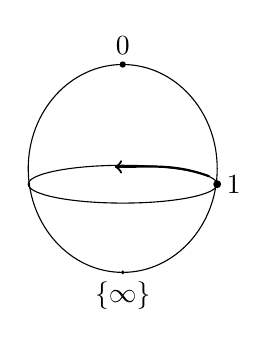
\begin{tikzpicture}
\draw (0,0) ellipse (1.2 and 1.32);
\draw (0,-.2) ellipse (1.2 and .24);
\draw[->,thick] (1.1,-.1) to[out=160,in=0] (-.1,.02);
\fill (0,1.32) circle (.04); \node[above] at (0,1.32) {$0$};
\fill (1.2,-.2) circle (.05); \node[right] at (1.2,-.2) {$1$};
\fill (0,-1.32) circle (.025); \node[below] at (0,-1.32) {$\unsure{\{\infty\}}$};
\end{tikzpicture}}
\deleted{\unsure{Il}}\inserted{Alors $X_1$} est un revêtement d'ordre $2$ de $X_0$\inserted{$=\mathbb P^1(\mathbb C)$}, ramifié \deleted{en dehors} au plus en $\{0,1,\infty\}$, (l'ordre du revêtement est le nb de repères \inserted{directs}, qui est $2$) avec
\[
\deleted{\unsure{\infty\longmapsto}}\qquad
g:\quad\begin{aligned}
1&\longmapsto0\\
-1&\longmapsto1\\
0,\infty&\longmapsto\infty
\end{aligned}
\]
ce qui épuise les fibres en $0,1,\infty$, et montre que la ramification est $2$ sur $0,1$, et pas de ramification sur $\infty$. \deleted{\unsure{Si l'on a}}\inserted{Pour} \unsure{avoir} la \deleted{\unsure{m}} situation analogue, \inserted{$g':\mathbb P^1(\mathbb C)\mathbin{-}\mathbb P^1(\mathbb C)$} mais avec
\[
g':\quad\begin{aligned}
0&\longmapsto0\\
\infty&\unsure{\longmapsto|\mathbin{-}}\infty\\
1,-1&\longmapsto1
\end{aligned}
\]
on aurait évidemment
\[
g'(z)=z^2,
\]
\margin{63}
